\documentclass{standalone}
\usepackage{tikz}
\usetikzlibrary{patterns, positioning}


\begin{document}
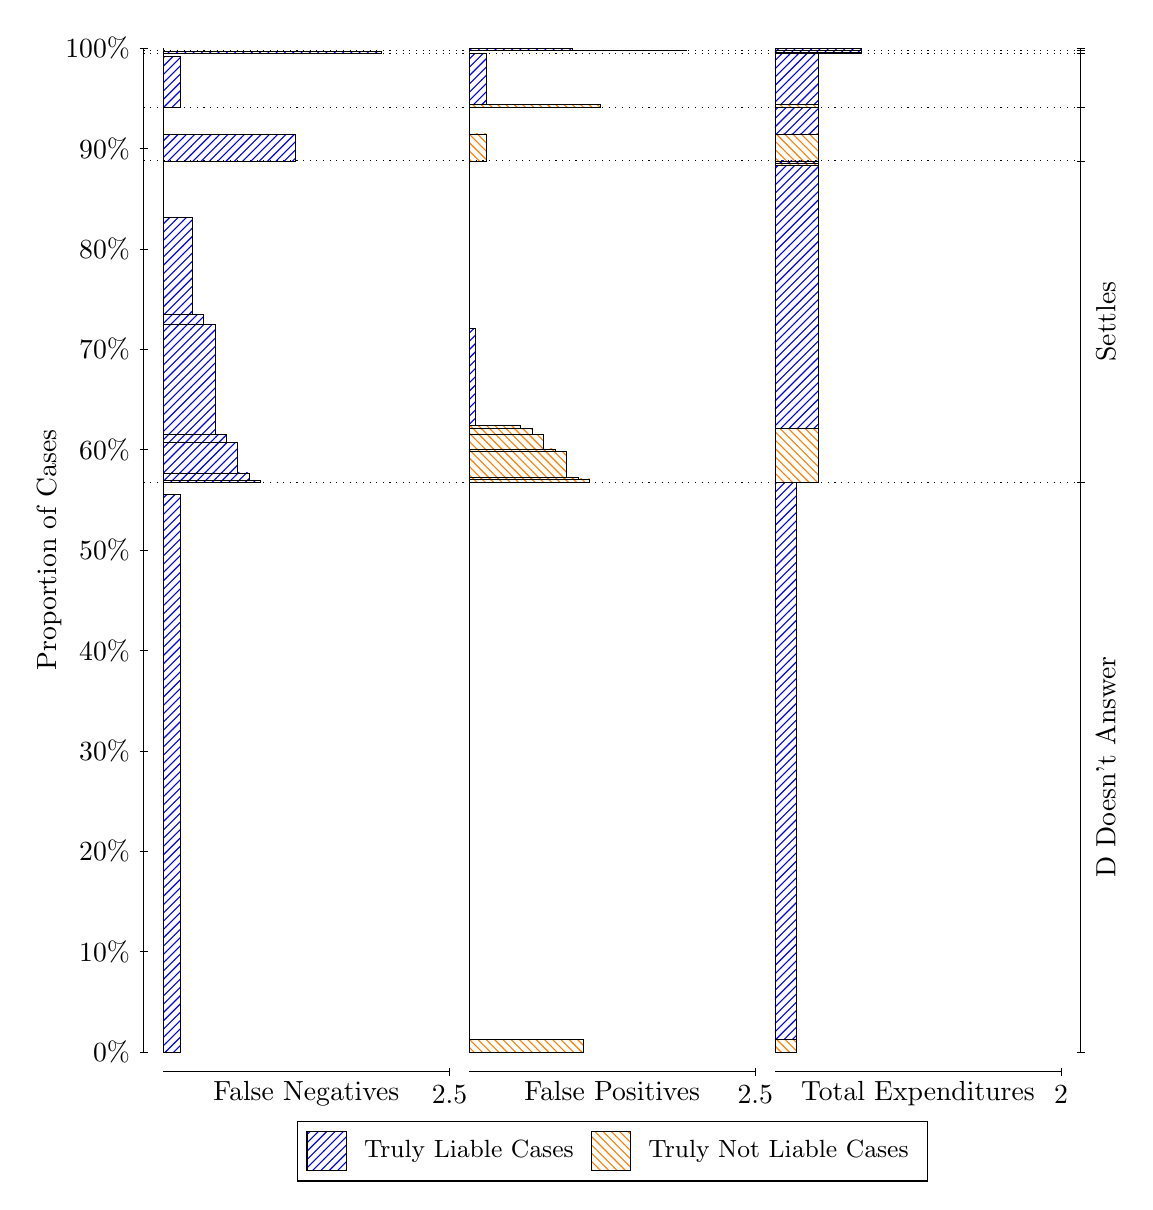
\begin{tikzpicture}
\draw[black, very thin] (1.5,1.75) -- (1.5,14.5);
\node[rotate=90, text=black, anchor=center] at (0.3, 8.125) {Proportion of Cases};
\draw[black, very thin] (1.45,1.75) -- (1.55,1.75);
\node[text=black, anchor=east] at (1.45, 1.75) {0\%};
\draw[black, very thin] (1.45,3.025) -- (1.55,3.025);
\node[text=black, anchor=east] at (1.45, 3.025) {10\%};
\draw[black, very thin] (1.45,4.3) -- (1.55,4.3);
\node[text=black, anchor=east] at (1.45, 4.3) {20\%};
\draw[black, very thin] (1.45,5.575) -- (1.55,5.575);
\node[text=black, anchor=east] at (1.45, 5.575) {30\%};
\draw[black, very thin] (1.45,6.85) -- (1.55,6.85);
\node[text=black, anchor=east] at (1.45, 6.85) {40\%};
\draw[black, very thin] (1.45,8.125) -- (1.55,8.125);
\node[text=black, anchor=east] at (1.45, 8.125) {50\%};
\draw[black, very thin] (1.45,9.4) -- (1.55,9.4);
\node[text=black, anchor=east] at (1.45, 9.4) {60\%};
\draw[black, very thin] (1.45,10.675) -- (1.55,10.675);
\node[text=black, anchor=east] at (1.45, 10.675) {70\%};
\draw[black, very thin] (1.45,11.95) -- (1.55,11.95);
\node[text=black, anchor=east] at (1.45, 11.95) {80\%};
\draw[black, very thin] (1.45,13.225) -- (1.55,13.225);
\node[text=black, anchor=east] at (1.45, 13.225) {90\%};
\draw[black, very thin] (1.45,14.5) -- (1.55,14.5);
\node[text=black, anchor=east] at (1.45, 14.5) {100\%};

\draw[black, very thin] (13.4,1.75) -- (13.4,14.5);
\draw[black, very thin] (13.35,1.75) -- (13.45,1.75);
\node[anchor=west] at (13.35, 1.75) {};
\draw[black, very thin] (13.35,8.9867) -- (13.45,8.9867);
\node[anchor=west] at (13.35, 8.9867) {};
\draw[black, very thin] (13.35,13.068) -- (13.45,13.068);
\node[anchor=west] at (13.35, 13.068) {};
\draw[black, very thin] (13.35,13.745) -- (13.45,13.745);
\node[anchor=west] at (13.35, 13.745) {};
\draw[black, very thin] (13.35,14.434) -- (13.45,14.434);
\node[anchor=west] at (13.35, 14.434) {};
\draw[black, very thin] (13.35,14.469) -- (13.45,14.469);
\node[anchor=west] at (13.35, 14.469) {};
\draw[black, very thin] (13.35,14.5) -- (13.45,14.5);
\node[anchor=west] at (13.35, 14.5) {};

\draw[black, very thin, pattern color=blue, pattern=north east lines] (1.75,1.75) rectangle (1.968,8.8282);
\draw[black, very thin, pattern color=orange, pattern=north west lines] (1.75,8.8282) rectangle (1.75,8.9867);
\draw[black, very thin, pattern color=blue, pattern=north east lines] (1.75,8.9867) rectangle (2.9853,9.0129);
\draw[black, very thin, pattern color=blue, pattern=north east lines] (1.75,9.0129) rectangle (2.84,9.1033);
\draw[black, very thin, pattern color=blue, pattern=north east lines] (1.75,9.1033) rectangle (2.6947,9.494);
\draw[black, very thin, pattern color=blue, pattern=north east lines] (1.75,9.494) rectangle (2.5493,9.5952);
\draw[black, very thin, pattern color=blue, pattern=north east lines] (1.75,9.5952) rectangle (2.404,10.992);
\draw[black, very thin, pattern color=blue, pattern=north east lines] (1.75,10.992) rectangle (2.2587,11.114);
\draw[black, very thin, pattern color=blue, pattern=north east lines] (1.75,11.114) rectangle (2.1133,12.348);
\draw[black, very thin, pattern color=orange, pattern=north west lines] (1.75,12.348) rectangle (1.75,13.068);
\draw[black, very thin, pattern color=blue, pattern=north east lines] (1.75,13.068) rectangle (3.4213,13.402);
\draw[black, very thin, pattern color=orange, pattern=north west lines] (1.75,13.402) rectangle (1.75,13.745);
\draw[black, very thin, pattern color=blue, pattern=north east lines] (1.75,13.745) rectangle (1.968,14.391);
\draw[black, very thin, pattern color=orange, pattern=north west lines] (1.75,14.391) rectangle (1.75,14.434);
\draw[black, very thin, pattern color=blue, pattern=north east lines] (1.75,14.434) rectangle (4.5113,14.46);
\draw[black, very thin, pattern color=orange, pattern=north west lines] (1.75,14.46) rectangle (1.75,14.469);
\draw[black, very thin, pattern color=orange, pattern=north west lines] (1.75,14.469) rectangle (1.75,14.472);
\draw[black, very thin, pattern color=blue, pattern=north east lines] (1.75,14.472) rectangle (1.75,14.5);
\draw[black, very thin, pattern color=orange, pattern=north west lines] (5.6333,1.75) rectangle (7.0867,1.9085);
\draw[black, very thin, pattern color=blue, pattern=north east lines] (5.6333,1.9085) rectangle (5.6333,8.9867);
\draw[black, very thin, pattern color=orange, pattern=north west lines] (5.6333,8.9867) rectangle (7.1593,9.0281);
\draw[black, very thin, pattern color=orange, pattern=north west lines] (5.6333,9.0281) rectangle (7.014,9.0486);
\draw[black, very thin, pattern color=orange, pattern=north west lines] (5.6333,9.0486) rectangle (6.8687,9.3802);
\draw[black, very thin, pattern color=orange, pattern=north west lines] (5.6333,9.3802) rectangle (6.7233,9.4082);
\draw[black, very thin, pattern color=orange, pattern=north west lines] (5.6333,9.4082) rectangle (6.578,9.5921);
\draw[black, very thin, pattern color=orange, pattern=north west lines] (5.6333,9.5921) rectangle (6.4327,9.6709);
\draw[black, very thin, pattern color=orange, pattern=north west lines] (5.6333,9.6709) rectangle (6.2873,9.7062);
\draw[black, very thin, pattern color=blue, pattern=north east lines] (5.6333,9.7062) rectangle (5.706,10.94);
\draw[black, very thin, pattern color=blue, pattern=north east lines] (5.6333,10.94) rectangle (5.6333,13.068);
\draw[black, very thin, pattern color=orange, pattern=north west lines] (5.6333,13.068) rectangle (5.8513,13.41);
\draw[black, very thin, pattern color=blue, pattern=north east lines] (5.6333,13.41) rectangle (5.6333,13.745);
\draw[black, very thin, pattern color=orange, pattern=north west lines] (5.6333,13.745) rectangle (7.3047,13.788);
\draw[black, very thin, pattern color=blue, pattern=north east lines] (5.6333,13.788) rectangle (5.8513,14.434);
\draw[black, very thin, pattern color=orange, pattern=north west lines] (5.6333,14.434) rectangle (5.6333,14.443);
\draw[black, very thin, pattern color=blue, pattern=north east lines] (5.6333,14.443) rectangle (5.6333,14.469);
\draw[black, very thin, pattern color=orange, pattern=north west lines] (5.6333,14.469) rectangle (8.3947,14.472);
\draw[black, very thin, pattern color=blue, pattern=north east lines] (5.6333,14.472) rectangle (6.9413,14.5);
\draw[black, very thin, pattern color=orange, pattern=north west lines] (9.5167,1.75) rectangle (9.7892,1.9085);
\draw[black, very thin, pattern color=blue, pattern=north east lines] (9.5167,1.9085) rectangle (9.7892,8.9867);
\draw[black, very thin, pattern color=orange, pattern=north west lines] (9.5167,8.9867) rectangle (10.062,9.6709);
\draw[black, very thin, pattern color=blue, pattern=north east lines] (9.5167,9.6709) rectangle (10.062,13.006);
\draw[black, very thin, pattern color=orange, pattern=north west lines] (9.5167,13.006) rectangle (10.062,13.042);
\draw[black, very thin, pattern color=blue, pattern=north east lines] (9.5167,13.042) rectangle (10.062,13.068);
\draw[black, very thin, pattern color=orange, pattern=north west lines] (9.5167,13.068) rectangle (10.062,13.41);
\draw[black, very thin, pattern color=blue, pattern=north east lines] (9.5167,13.41) rectangle (10.062,13.745);
\draw[black, very thin, pattern color=orange, pattern=north west lines] (9.5167,13.745) rectangle (10.062,13.788);
\draw[black, very thin, pattern color=blue, pattern=north east lines] (9.5167,13.788) rectangle (10.062,14.434);
\draw[black, very thin, pattern color=orange, pattern=north west lines] (9.5167,14.434) rectangle (10.607,14.443);
\draw[black, very thin, pattern color=blue, pattern=north east lines] (9.5167,14.443) rectangle (10.607,14.469);
\draw[black, very thin, pattern color=orange, pattern=north west lines] (9.5167,14.469) rectangle (10.607,14.472);
\draw[black, very thin, pattern color=blue, pattern=north east lines] (9.5167,14.472) rectangle (10.607,14.5);
\draw[black, dotted] (1.5,8.9867) -- (13.4,8.9867);
\draw[black, dotted] (1.5,13.068) -- (13.4,13.068);
\draw[black, dotted] (1.5,13.745) -- (13.4,13.745);
\draw[black, dotted] (1.5,14.434) -- (13.4,14.434);
\draw[black, dotted] (1.5,14.469) -- (13.4,14.469);
\draw[black, very thin] (1.75,1.5) -- (5.3833,1.5);
\node[text=black, anchor=north] at (3.5667, 1.5) {False Negatives};
\draw[black, very thin] (5.3833,1.45) -- (5.3833,1.55);
\node[text=black, anchor=north] at (5.3833, 1.45) {2.5};

\draw[black, very thin] (5.6333,1.5) -- (9.2667,1.5);
\node[text=black, anchor=north] at (7.45, 1.5) {False Positives};
\draw[black, very thin] (9.2667,1.45) -- (9.2667,1.55);
\node[text=black, anchor=north] at (9.2667, 1.45) {2.5};

\draw[black, very thin] (9.5167,1.5) -- (13.15,1.5);
\node[text=black, anchor=north] at (11.333, 1.5) {Total Expenditures};
\draw[black, very thin] (13.15,1.45) -- (13.15,1.55);
\node[text=black, anchor=north] at (13.15, 1.45) {2};

\node[text=black, centered, rotate=90] at (13.72, 5.3684) {D Doesn't Answer};
\node[text=black, centered, rotate=90] at (13.72, 11.027) {Settles};





\draw (7.449999999999999,1.5) node[draw=none] (baseCoordinate) {};
\begin{scope}[align=center]
        \matrix[scale=0.5, draw=black, below=0.5cm of baseCoordinate, nodes={draw}, column sep=0.1cm]{
            \node[rectangle, draw, minimum width=0.5cm, minimum height=0.5cm, pattern color=blue, pattern=north east lines] {}; &
            \node[draw=none, font=\small, text=black] (B) {Truly Liable Cases}; &
            \node[rectangle, draw, minimum width=0.5cm, minimum height=0.5cm, pattern color=orange, pattern=north west lines] {}; &
            \node[draw=none, font=\small, text=black] (B) {Truly Not Liable Cases}; \\
            };
\end{scope}

\end{tikzpicture}
\end{document}